\documentclass[11pt,a4paper]{article}

\usepackage[utf8]{inputenc}
\usepackage[T1]{fontenc}
\usepackage{lmodern}
\usepackage[polish]{babel}
\usepackage[a4paper,margin=2.5cm]{geometry}
\usepackage{graphicx}
\usepackage[hypertexnames=false]{hyperref}
\usepackage{amsmath,amssymb}
\usepackage{textcomp}
\usepackage{enumitem}
\usepackage{booktabs}
\setlength{\parindent}{0pt}

\newcommand{\coursename}{Reprezentacja Wiedzy}
\newcommand{\projecttitle}{Procesy działań złożonych\\[0.3em]
  \Large Instrukcja użytkownika}
\newcommand{\projectdate}{Warszawa, 11 czerwca 2026}

\begin{document}
\sloppy

\begin{titlepage}
    \centering

    
\includegraphics[width=0.8\textwidth]{imgs/politechnika.png}\par
    \vspace{2.5cm}

    {\Large \coursename\par}
    \vspace{1.2cm}

    {\Huge \bfseries \projecttitle \par}
    \vspace{2cm}

    {\Large Zespół projektowy nr~4:\par}
    \vspace{0.5cm}
    {\large
        Wojciech Jasiński (koordynator)\\[0.2em]
        Krzysztof Gryboś\\[0.2em]
        Jarosław Bieniek\\[0.2em]
        Filip Filipkowski\\[0.2em]
        Sebastian Rydz\\[0.2em]
        Jakub Pietrzak\\[0.2em]
        Sandra Adamiec\par
    }

    \vfill

    {\large \projectdate\par}
\end{titlepage}

% ══════════════════════════════════════════════════════════════════
\section{Uruchomienie}

Gotowe pliki znajdują się w~katalogu \texttt{app/release/}. Są
samowystarczalne --- nie wymagają instalowania platformy .NET.

\begin{itemize}
  \item \textbf{Windows:} dwuklik na \texttt{Ds4.Gui.exe}.
  \item \textbf{Linux:} plik \texttt{Ds4.CrossGui}
        (w~razie potrzeby \texttt{chmod +x Ds4.CrossGui}, potem
        \texttt{./Ds4.CrossGui}).
\end{itemize}

Katalog \texttt{examples/} musi pozostać obok pliku wykonywalnego ---
z~niego program wczytuje listę wbudowanych przykładów.

Uruchomienie ze źródeł (wymaga .NET~8 SDK): w~katalogu \texttt{app/}
skrypt \texttt{RUN\_GUI.bat} (Windows) albo \texttt{RUN\_CROSS\_GUI.sh}
(Linux/macOS).

% ══════════════════════════════════════════════════════════════════
\section{Okno programu}

\begin{center}
  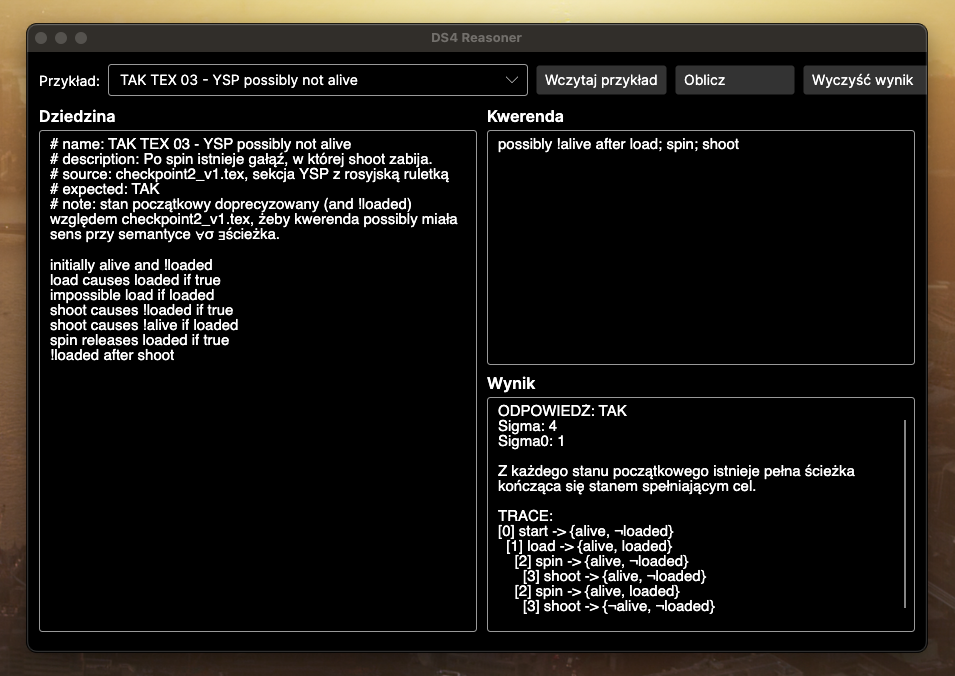
\includegraphics[width=0.95\textwidth]{imgs/ui.png}
\end{center}

Okno ma cztery elementy:

\begin{enumerate}
  \item \textbf{Pasek przykładów} (góra) --- lista rozwijana z~57 wbudowanymi
        przypadkami oraz przyciski \emph{Wczytaj przykład}, \emph{Oblicz}
        i~\emph{Wyczyść wynik}.
  \item \textbf{Dziedzina} (lewy panel) --- edytowalny opis dziedziny
        w~języku akcji (rozdział~\ref{sec:dziedzina}).
  \item \textbf{Kwerenda} (prawy górny panel) --- jedno pytanie do dziedziny
        (rozdział~\ref{sec:kwerenda}).
  \item \textbf{Wynik} (prawy dolny panel) --- odpowiedź wraz z~uzasadnieniem
        i~przebiegiem wykonania (rozdział~\ref{sec:wynik}).
\end{enumerate}

Typowa praca: wybierz przykład i~kliknij \emph{Wczytaj przykład} (albo wpisz
własną dziedzinę i~kwerendę), następnie kliknij \emph{Oblicz}.

% ══════════════════════════════════════════════════════════════════
\section{Jak opisać dziedzinę}
\label{sec:dziedzina}

Dziedzinę opisuje się zdaniami --- po jednym w~wierszu. Wiersze zaczynające
się od~\texttt{\#} to komentarze. Nazwy fluentów i~akcji program zbiera sam
z~treści zdań (deklaracje \texttt{fluents}/\texttt{actions} są opcjonalne).
Poniżej opis dziedziny ,,rosyjskiej ruletki'' budowany krok po kroku.

\textbf{Stan początkowy.} Postać na początku żyje --- o~nabiciu broni nic
nie mówimy, więc oba przypadki będą brane pod uwagę:
\begin{verbatim}
initially alive
\end{verbatim}

\textbf{Efekt akcji} --- \texttt{causes \dots\ if \dots}. Strzał zabija,
ale tylko gdy broń jest nabita:
\begin{verbatim}
shoot causes not alive if loaded
load causes loaded if not loaded
\end{verbatim}

\textbf{Efekt niedeterministyczny} --- \texttt{releases}. Zakręcenie bębenkiem
sprawia, że \texttt{loaded} może wyjść dowolnie:
\begin{verbatim}
spin releases loaded if true
\end{verbatim}

\textbf{Niewykonalność} --- \texttt{impossible \dots\ if \dots}. Nie można
nabić broni już nabitej:
\begin{verbatim}
impossible load if loaded
\end{verbatim}

\textbf{Ograniczenie stałe} --- \texttt{always}. Gdyby w~dziedzinie były
fluenty powiązane (np. $p$ zawsze pociąga $q$), zapisalibyśmy:
\begin{verbatim}
always p implies q
\end{verbatim}
Takie ograniczenie działa we wszystkich stanach i~wymusza skutki uboczne
akcji.

W~formułach (warunkach \texttt{if}, \texttt{initially}, \texttt{always},
celach kwerend) używa się wyłącznie operatorów słownych: \texttt{not}~(nie),
\texttt{and}, \texttt{or}, \texttt{implies}, \texttt{iff} oraz stałych
\texttt{true}/\texttt{false}. Program nie przyjmuje symboli
(\texttt{!}, \texttt{\&}, \texttt{|}, \texttt{->}, \texttt{<->}) --- zgłasza wtedy błąd.

% ══════════════════════════════════════════════════════════════════
\section{Jak zadać kwerendę}
\label{sec:kwerenda}

Kwerenda to jedno zdanie. Pytamy o~\emph{proces}, czyli ciąg kroków
rozdzielonych średnikami; w~jednym kroku może wykonywać się równocześnie
kilka akcji --- zapisuje się je w~nawiasach klamrowych:

\begin{verbatim}
spin; shoot              (dwa kroki po jednej akcji)
{lift_a, lift_b}; carry  (dwie akcje naraz, potem jedna)
\end{verbatim}

Cztery rodzaje pytań:

\begin{center}
\small
\begin{tabular}{@{}ll@{}}
\toprule
\textbf{Zapis} & \textbf{Znaczenie} \\
\midrule
\texttt{possibly executable after P}  & czy proces $P$ \emph{kiedykolwiek} da się wykonać do końca \\
\texttt{necessary executable after P} & czy proces $P$ da się wykonać \emph{zawsze} \\
\texttt{possibly}~$\gamma$~\texttt{after P}  & czy $P$ \emph{kiedykolwiek} prowadzi do celu $\gamma$ \\
\texttt{necessary}~$\gamma$~\texttt{after P} & czy $P$ \emph{zawsze} prowadzi do celu $\gamma$ \\
\bottomrule
\end{tabular}
\end{center}

,,Zawsze'' oznacza: dla każdego możliwego stanu początkowego i~każdego
przebiegu (przy niedeterminizmie); ,,kiedykolwiek'' --- że z~każdego
możliwego stanu początkowego istnieje przynajmniej jeden pełny przebieg.
Przykład:

\begin{verbatim}
possibly not alive after spin; shoot
\end{verbatim}

% ══════════════════════════════════════════════════════════════════
\section{Jak czytać wynik}
\label{sec:wynik}

Panel \emph{Wynik} zawiera kolejno:

\begin{itemize}
  \item \textbf{ODPOWIEDŹ: TAK / NIE} --- odpowiedź na kwerendę;
  \item \textbf{liczba stanów} --- liczbę stanów dopuszczalnych $|\Sigma|$
        (zgodnych z~\texttt{always}) oraz liczbę możliwych stanów
        początkowych $|\Sigma_0|$;
  \item \textbf{uzasadnienie} --- jedno--dwa zdania, np. wskazanie ścieżki
        (dla TAK przy \texttt{possibly}) albo kontrprzykładu (dla NIE przy
        \texttt{necessary});
  \item \textbf{TRACE} --- drzewo wykonań procesu. Każdy wiersz to jeden
        węzeł: numer kroku w~nawiasach kwadratowych, wykonywana akcja
        i~stan po niej (przedrostek \texttt{not} oznacza fluent fałszywy), np.
\begin{verbatim}
[0] start: {alive, not loaded}
  [1] spin: {alive, not loaded}
    [2] shoot: {alive, not loaded}
  [1] spin: {alive, loaded}
    [2] shoot: {not alive, loaded}
\end{verbatim}
        Wcięcie oznacza kolejny krok procesu; rozgałęzienie --- kilka możliwych
        wyników (niedeterminizm). Wiersz \texttt{BLOCKED: brak następników dla
        kolejnego kroku procesu} oznacza, że w~tym miejscu akcji nie dało się
        wykonać i~ścieżka się urywa.
\end{itemize}

\textbf{Sprzeczny opis.} Jeżeli dziedzina jest sprzeczna, program nie pokazuje
odpowiedzi TAK/NIE ani śladu, lecz komunikat o~błędzie:
\begin{itemize}
  \item sprzeczne ograniczenia \texttt{always} (żaden stan ich nie spełnia,
        $|\Sigma| = 0$) --- \texttt{BŁĄD: Model jest pusty: ograniczenia always
        są sprzeczne.};
  \item sprzeczny opis początkowy --- gdy zdania \texttt{initially},
        \texttt{after} lub \texttt{observable after} nie mogą zostać spełnione
        jednocześnie ($|\Sigma_0| = 0$) --- \texttt{BŁĄD: Brak stanów
        początkowych: initially/after/observable after są sprzeczne.}
\end{itemize}
W~obu przypadkach należy poprawić opis dziedziny.

% ══════════════════════════════════════════════════════════════════
\section{Przykłady i~praca z~plikami}

\textbf{Wbudowane przykłady.} Lista na pasku górnym zawiera 57 przypadków.
Prefiks \texttt{tak\_}/\texttt{nie\_} mówi, jaka jest poprawna odpowiedź,
a~komentarze na początku dziedziny opisują, co dany przykład pokazuje.

\textbf{Format plików.} Każdy przykład to trzy pliki tekstowe o~wspólnej
nazwie:
\begin{itemize}
  \item \texttt{<id>.domain} --- opis dziedziny,
  \item \texttt{<id>.query} --- jedna kwerenda,
  \item \texttt{<id>.expected} --- oczekiwana odpowiedź (używana przez testy).
\end{itemize}
Własne przykłady wystarczy dograć do katalogu \texttt{examples/} ---
po ponownym uruchomieniu pojawią się na liście.

\textbf{Wersja konsolowa.} Te same obliczenia można wykonać bez GUI
(wymaga .NET~8 SDK, katalog \texttt{app/}):
\begin{verbatim}
dotnet run --project src/Ds4.Cli -- plik.domain plik.query
\end{verbatim}
Opcja \texttt{-{}-examples} wypisuje listę wbudowanych przykładów,
a~\texttt{-{}-example <id>} rozwiązuje wskazany przykład.

\end{document}
